\documentclass{article}
\usepackage{graphicx}
\usepackage{listings} % nice code layout
\usepackage[section]{placeins}
\usepackage{xcolor}
\usepackage[utf8]{inputenc}
\lstset{language = Verilog}
\lstset{language = C++}
\graphicspath{ {./img/} }


\usepackage[a4paper, margin=1.25in]{geometry}


\author{Justin Bui}
\title{Microblaze Implementation of a Multicolored LED Control System}

\begin{document}

\maketitle
\newpage

\tableofcontents
\newpage

\section{Introduction}
This document outlines the design and implementation for my final project for ELC 5396. This project makes use of the Digilent NEXYS 4 Artix-7 FPGA development board to implement a Microblaze based multicolored LED control system. The document below includes the functional discription, code portions, and thought process behind the systems design and implementation, as well as some additional features that were not developed due to issues with compiler version issues 

\section{Project Description}
The Multicolored LED control system is designed to highlight the flexibility of developing softcore systems. Based on the 32bit Microblaze softcore, built on the Artix-7, this project provides a base foundation for the development of more advanced features. The core functionality of this project allows for the control of the two RGB LEDs present on the Nexys 4 DDR development board. Each LED color can be set or cleared independently, and tied to a variety of control mechanisms.


\begin{table}[h!]
	\begin{center}
		\caption{Color Configurations}
		\label{table:table1}
		\begin{tabular}{l l l}
			\textbf{Color} & \textbf{RGB Values} \\
			\hline
			Off  &  0 0 0 \\
			Red & 1 0 0 \\
			Green & 0 1 0 \\
			Blue & 0 0 1 \\
			Yellow & 1 1 0 \\
			Cyan & 0 1 1 \\
			Purple & 1 0 1 \\
			White & 1 1 1 
		\end{tabular}
	\end{center}
\end{table}

\section{Thought Process}
I came up with the idea to build out this application while working on implementing a PDM controller for the onboard microphone. I first included one of the multicolored LEDs to assist with state and value tracking. After some difficulties in successfully converting the pulsed data to a tangible audio signal, I decided to switch gears and write a core and wrapper to make use of the RGB LEDs as troubleshooting and and status indicators. 

Much of this idea stems from my past work experience, as both a product development and applications engineer. Status LEDs provide a surprisingly large benefit, given their relative simplicity. I've written the core to allow for the setting and clearing of specific colors independently, allowing for various implementations. Each LED can be individually configured to display the colors as seen in above. The core's functionality can be expanded to include light intensity control (via pwm), Pulse frequency (for communications indicators), etc.

	\begin{figure}[h!]
		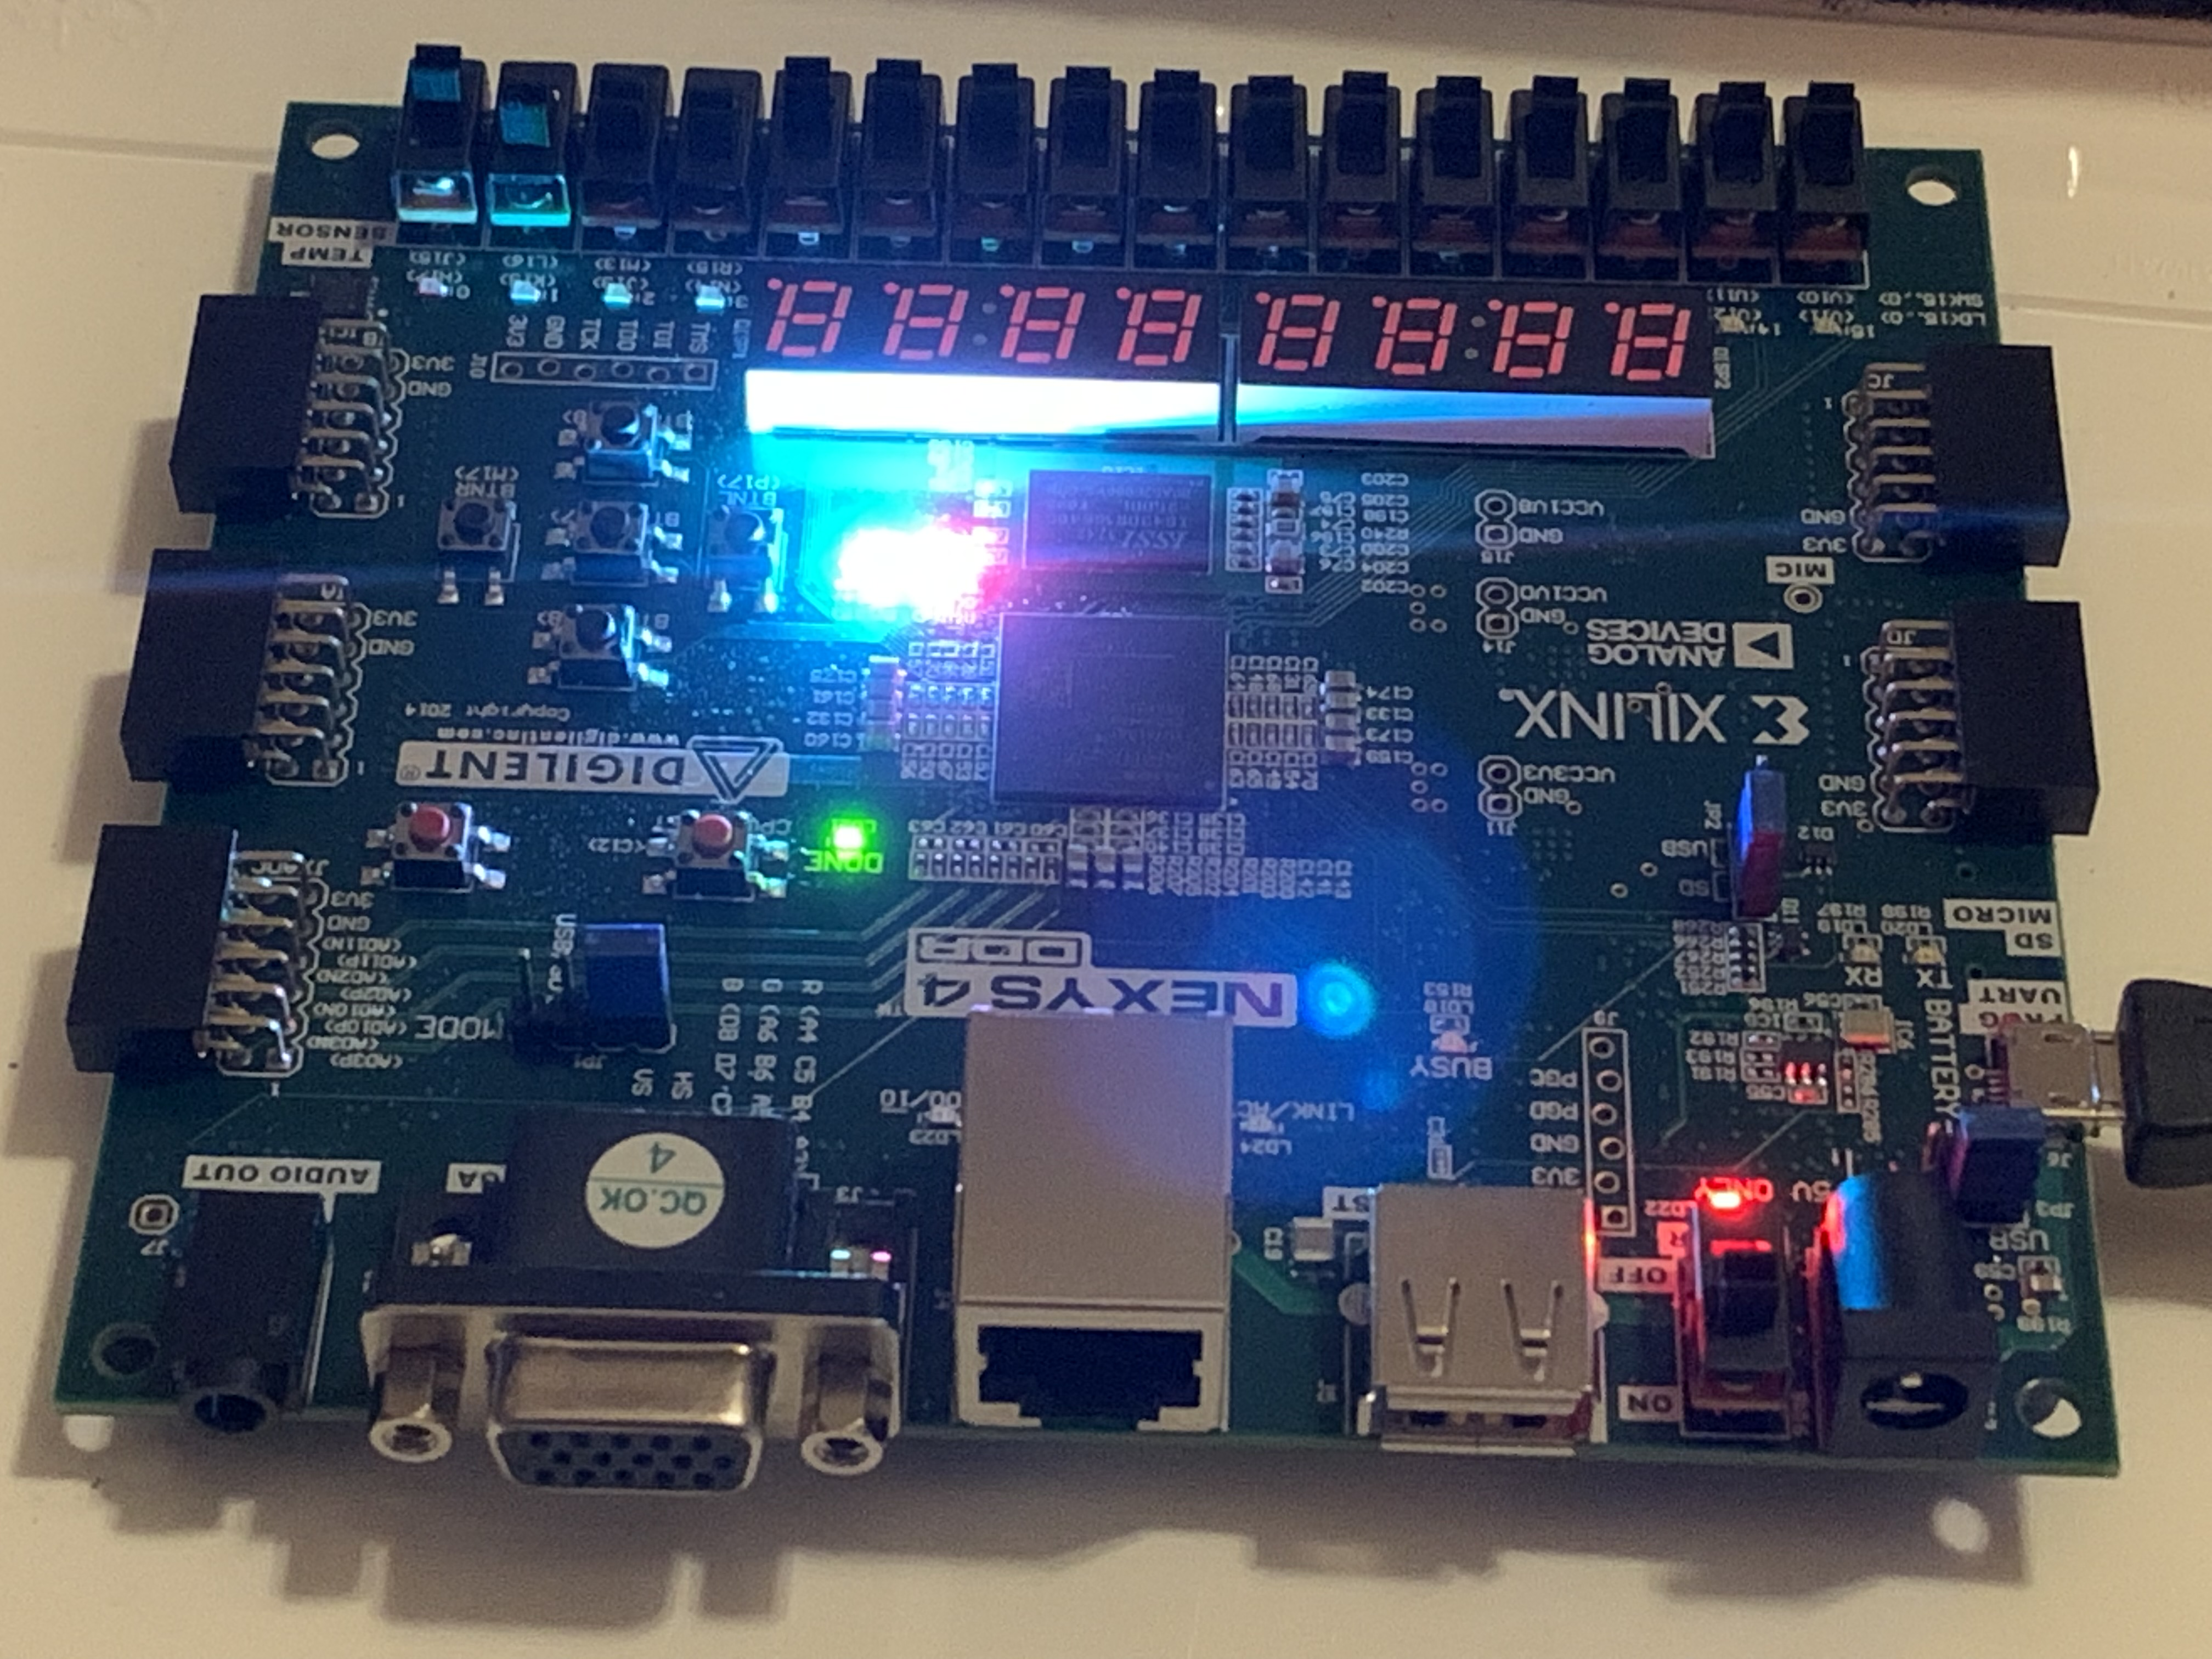
\includegraphics[width=.9\linewidth]{cr.JPG}
		\caption{Example: Cyan and Yellow LED Configurations}
	\end{figure}

\newpage

\section{Core Code}
The core functionality of the RGB LED controller is reduced to two SystemVerilog files, called MLED.sv and bui\_mled\_core.sv. The MLED file creates the basic MLED (short for Multicolored LED) element, which consists of three inputs, r, g, and b for the corresponding independent LED colors, and a three bit output which corresponds to the "register" value for the LED. This code also handles in clocking in of the individual values via an input clock signal.

\begin{lstlisting}[language=Verilog]
module MLED(
        input logic clk, reset,
        input logic red, green, blue,
        output logic [2:0] led_out
    );
\end{lstlisting}

This MLED element is then passed along as a component of the core (bui\_mled\_core.sv). The core is responsible for generating two MLED elements (the Nexys 4 board has two RGB LEDs), as well as creating the wrapper function. The basic wrapper circuit consists of a register element which holds the values for each of the individual RGB elements in the LEDs. I have written this core such that each LED is represented by a Byte. For this implementation, the mled0 and mled1 components values are determined by the 3 least significant Bits of the least significant two Bytes of the data register (address 0x00).  This basic implementation allows for the configuration of the LED elements without complex addressing (which will be addressed below).

\newpage

\begin{lstlisting}[language = Verilog]
module bui_mled_core(
    // general signals
    input logic clk, reset,
    
    // slot interface
    input logic cs,
    input logic read,
    input logic write,
    input logic [4:0] addr,
    input logic [31:0] wr_data,
    output logic [31:0] rd_data,
    
    // LED Ports
    output logic [2:0] mled0, mled1
    );
    logic [31:0] data_reg;      // create a data register
    
    // Initialize both rbg LEDS
    // MLED 0 - Byte 0
    MLED led0 (.clk(clk), .reset(reset), .red(data_reg[0]), .green(data_reg[1]), 
               .blue(data_reg[2]), .led_out(mled0));
    // MLED 1 - Byte 1
    MLED led1 (.clk(clk), .reset(reset), .red(data_reg[8]), .green(data_reg[9]), 
                          .blue(data_reg[10]), .led_out(mled1));
                                         
    always_ff @(posedge clk, posedge reset)
        begin
            if(reset)
                data_reg <= 0;          // clear the data
            else
                data_reg <= wr_data;    // load in new data 
        end  
    assign rd_data = 0;     // read data currently not used 
endmodule
\end{lstlisting}



\section{Microblaze Implementation}
Now that the core has been built up, it must be integrated into the Microblaze. This is accomplished my implementing the wrapper described above into the mmio\_sys\_vanilla.sv file originally provided by Pong Chu. I have expanded the verilog header file to add a 14th slot for the MLED core. The code below ties the mled core to the mmio unit, which is ultimately tied to the cpu via the bridge code (also provided by Chu).

\newpage

\begin{lstlisting}[language=Verilog]
    // slot 14: Multicolored LED
    bui_mled_core led_slot14(
    .clk(clk),
    .reset(reset),
    .cs(cs_array[`S14_3LED]),
    .read(mem_rd_array[`S14_3LED]),
    .write(mem_wr_array[`S14_3LED]),
    .addr(reg_addr_array[`S14_3LED]),
    .rd_data(rd_data_array[`S14_3LED]),
    .wr_data(wr_data_array[`S14_3LED]),
    .mled0(rgb_led1),
    .mled1(rgb_led2)
    );
\end{lstlisting}

From here, we can begin to develop the software portion of the project.


\section{Software Implementation}
The software impelmentation for this project comprises some of the vanilla test project's code, which I have made use of as a debugging tool throughout development. The core code for this project surrounds the BUI\_3LED.h and BUI\_3LED.cpp files. The names are different simply due to the way development occured, there is no particular reason for the change in name. These files were programmed in a similar fashion to the GPIO\_Core code files. I have set up the constructor and fuctions in a way that allow for the individual configuration of each color and each led. Each of the set and clear functions takes an unsigned 8 bit integer argument as a pseudoaddress. I refer to this as a pseudoaddress simply because, as indicated previously, the least significant Byte is reserved for MLED0\/RGB\_LED1, and the 2nd Byte is reserved for MLED1\/RGB\_LED2. Each function then sets or clears the MLEDs specific color (Red, Green, or Blue). The code below shows the constructor and function prototypes for the mLED class.

\begin{lstlisting}[language=C++]
class mLED {
public:
	// Register Map
   enum {
      DATA_REG = 0 /**< input data register */
   };
   // Constructor / Destructor 
   mLED(uint32_t core_base_addr);
   ~mLED();                  // not used

   /* methods */
   uint32_t read();
   void write(uint32_t data);
   // set color function
   void setRed(uint8_t led);
   void setGreen(uint8_t led);
   void setBlue(uint8_t led);
   // clear color function
   void clrRed(uint8_t led);
   void clrGreen(uint8_t led);
   void clrBlue(uint8_t led);

private:
   uint32_t base_addr;
   uint32_t wr_data;
};
\end{lstlisting}

\newpage
As you can see, the provided functionality for this project is straight forward. Simply set or clear the particular color for the led that is passed into the function. Below is the code for both setRed and clrRed, the Green and Blue functions are written in a similar fashion.

\begin{lstlisting}[language=C++]
// Set Red LED Bit (1 or 9)
void mLED::setRed(uint8_t led) {
	uint32_t red;
	if(led==1)
		red=0x100;
	else
		red=0x1;
	write(red);
}

// Clear Red LED Bit
void mLED::clrRed(uint8_t led){
	uint32_t dat = read();
	if(led==1)
		write(dat & ~0x100);
	else
		write(dat & ~0x1);
}
\end{lstlisting}

These functions were tested by strobing through different colors using the mled\_check function (shown below). The functionality here can be expanded to use the LEDs for a variety of functions, including strobing during UART communications, indicate battery charge status\/level, etc.

\begin{lstlisting}[language=C++]
void mled_check(mLED *mled_p) {
	int i;
	for (i = 0; i < 5	; i++)
	{
		mled_p->setRed(0);
		sleep_ms(1000);
		uart.disp("led red \n");
		mled_p->setGreen(0);
		sleep_ms(500);
		uart.disp("led green\n");
		mled_p->clrRed(0);
		sleep_ms(500);
		mled_p->setBlue(1);
		sleep_ms(500);
		mled_p->clrGreen(0);
		sleep_ms(500);
		uart.disp("led blue\n");
		mled_p->clrBlue(1);
		sleep_ms(500);
	}
}
\end{lstlisting}

\end{document}